\documentclass[titlepage, 11pt]{article}
\usepackage[a4paper, total={6in, 9.5in}]{geometry}
\usepackage{graphicx}
\usepackage{amsmath,amsfonts,amssymb}
\usepackage{listings}
\usepackage{booktabs}
\usepackage[T1]{fontenc}
\usepackage{listings}
\usepackage{color}
\usepackage{minted}
\usepackage[colorlinks=true, linkcolor=blue, urlcolor=blue, citecolor=blue, pdfborder={0 0 255}]{hyperref}
\usepackage{colortbl}
\usepackage{url}
\usepackage{xcolor}
\usepackage{caption}
\usepackage{subcaption}
\usepackage{dirtytalk}
\usepackage[semicolon, round]{natbib}
\usepackage[ruled]{algorithm2e}
\captionsetup[table]{skip=10pt}
\renewcommand{\vec}[1]{\mathbf{#1}}
\SetKwComment{Comment}{$\triangleright$\ }{}
% \hypersetup{%
% 	colorlinks=true,
% 	linkcolor=blue,
% 	linkbordercolor={0 0 1}
% }

% \renewcommand\lstlistingname{Algorithm}
% \renewcommand\lstlistlistingname{Algorithms}
% \def\lstlistingautorefname{Alg.}

% \lstdefinestyle{Python}{
% 	language        = Python,
% 	frame           = lines, 
% 	basicstyle      = \footnotesize,
% 	keywordstyle    = \color{blue},
% 	stringstyle     = \color{green},
% 	commentstyle    = \color{red}\ttfamily
% }

% \setlength{\parindent}{0.0in}
% \setlength{\parskip}{0.05in}

\newcommand{\argmin}{\mathop{\mathrm{argmin}}}
\newcommand{\argmax}{\mathop{\mathrm{argmax}}}
\newcommand{\minimize}{\mathop{\mathrm{minimize}}}
\newcommand{\maximize}{\mathop{\mathrm{maximize}}}
\newcommand{\st}{\mathop{\mathrm{subject\,\,to}}}
\newcommand{\dist}{\mathop{\mathrm{dist}}}
\newcommand{\norm}[1]{\left\lVert#1\right\rVert}
\renewcommand{\vec}[1]{\mathbf{#1}}

\def\R{\mathbb{R}}
\def\E{\mathbb{E}}
\def\P{\mathbb{P}}
\def\S{\mathbb{S}}
\def\Cov{\mathrm{Cov}}
\def\Var{\mathrm{Var}}
\def\half{\frac{1}{2}}
\def\quat{\frac{1}{4}}
\def\sign{\mathrm{sign}}
\def\supp{\mathrm{supp}}
\def\th{\mathrm{th}}
\def\tr{\mathrm{tr}}
\def\dim{\mathrm{dim}}
\def\dom{\mathrm{dom}}

\title{
{EE1103: Numerical Methods} \\~\\
{\vlarge Programming Assignment {\#} 4}\\
}\author{ANIRUDH B S, EE21B019\\
Collaborators: & AMIZHTHNI P R K, EE21B015
 & ANKITA HARSHA MURTHY, EE21B020}
\date{\today}

\begin{document}
\maketitle

\setcounter{page}{0}
\tableofcontents
\listoffigures
\newpage

\section{Problem 1}
\noindent The aim of this exercise is to model a system of linear equations and solve the same using \textbf{Gauss elimination}. Fig.~\ref{fig:circuit} depicts an electrical circuit with \textit{four} nodes, namely, one reference node and three nodes with unknown voltages marked $v_1$, $v_2$ and $v_3$. The voltage at the reference node is $0$ V. The current sources and resistors have designated values and are marked on the schematic. The unknown voltages $v_1$, $v_2$ and $v_3$ can be determined using KCL.
\begin{itemize}
    \item [(a)] Construct KCL equations for each of the three nodes. Note that these equations are to be written in terms of the current sources and the current through each resistor.
    \item [(b)] Write a routine in C/C++ that implements Gauss elimination to solve for $v_1$, $v_2$ and $v_3$. In your report, paste a screenshot of the output displayed in your console. 
\end{itemize}
\begin{figure}[h]
    \centering
    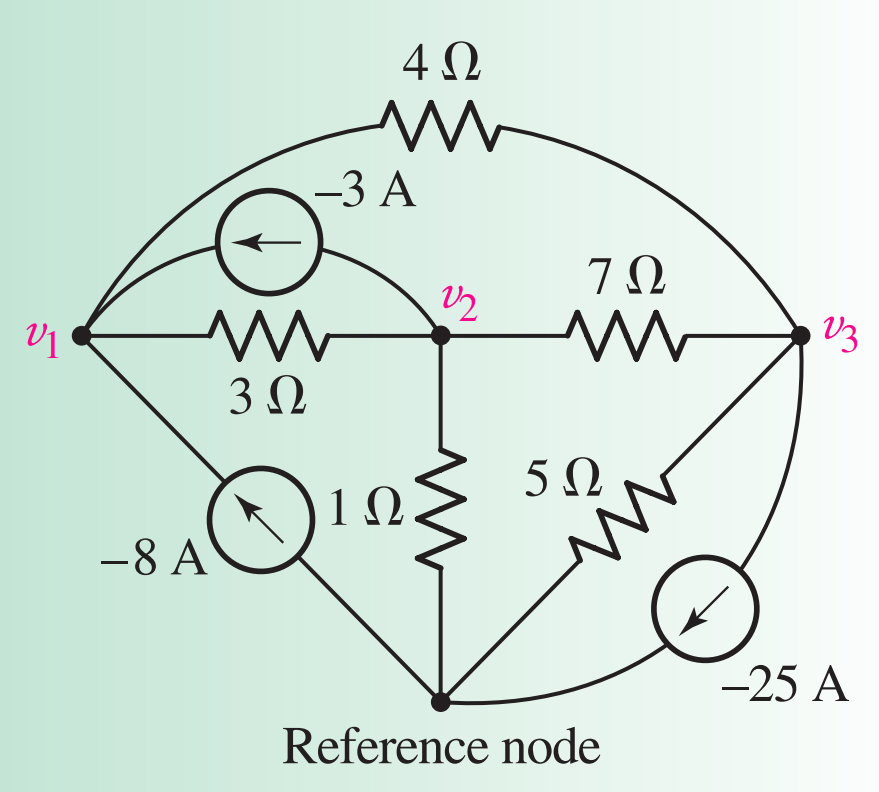
\includegraphics[scale = 0.17]{circuit.png}
    \caption{Circuit diagram}
    \label{fig:circuit}
\end{figure}

\subsection{Approach}
 In this problem, I shall use Gaussian Elimination to obtain the solutions of a system of linear equations that possesses a unique solution. 
%%%%%%%%%%%%%%%%%%%%%%%%%%%%%%%%%%%%%%%%%%%%%%%%%%%%%%

\subsection{Algorithm}
In this section, I present the pseudocode/flowchart of the algorithm used to solve the problem.

The pseudocode for the summation is provided in Algorithm~\ref{alg1}.
\begin{center}
\begin{algorithm}[H]\label{alg1}

\SetAlgoLined
{
\underline{\textbf{Gaussian Elimination} }\\{
\For{$j=1$ to $n-1$}{
   \For{$i=j+1$ to n}{
   \If{$a_{ij}==0$}{
       break \\ 
   }
      $r_{ij}$ $\gets$ $\frac{a_{ij}}{a_{jj}}$ \\
      \For{$k=j+1$ to n}{
         $a_{ik}$ $\gets$ $a_{ik} - r_{ij}a_{jk}$ \\
      }
      $b_{i}$ $\gets$ $b_{i}-r_{ij}b{j}$ \\
   }
}
}
\underline{\textbf{Back Substitution}} \\{
    \If{$u_{nn}==0$}{
       break \\ 
   }
    Set $x_n = {y_n}/{u_{nn}}$ \\
    \For{$i=n-1$ to 1}{
      ${x_i \gets (y_i - \sum_{j=i+1}^{n}u_{ij}x_j)/u_{ii}}$
    }
}
}
 \caption{Gaussian Elimination}
\end{algorithm}    
\end{center}

%%%%%%%%%%%%%%%%%%%%%%%%%%%%%%%%%%%%%%%%%%%%%%%%%%%%%%
\subsection{Results}

In this section, I shall paste the screenshots of the Matrices obtained after Gaussian Elimination. 

The set of linear equations that needs to be solved after writing down the Kirchoff's Circuital Law is :

\begin{equation}
    0.5833 v_1 - 0.3333 v_2 - 0.25 v_3 = -11
\end{equation}
\begin{equation}
    -0.3333 v_1 + 1.4762 v_2 - 0.1429 v_3 = 3
\end{equation}
\begin{equation}
    -0.25 v_1 - 0.1429 v_2 + 0.5929 v_3 = 25
\end{equation}

The values of the voltages I obtained after solving the system of linear equations using Gaussian Elimination are as follows. 
\begin{itemize}
    \item [1] $V_1 = 5.412425$
    \item [2] $V_2 = 7.737463$
    \item [3] $V_3 = 46.312683$
\end{itemize}

\begin{figure}[!tbh]
  	\centering
  	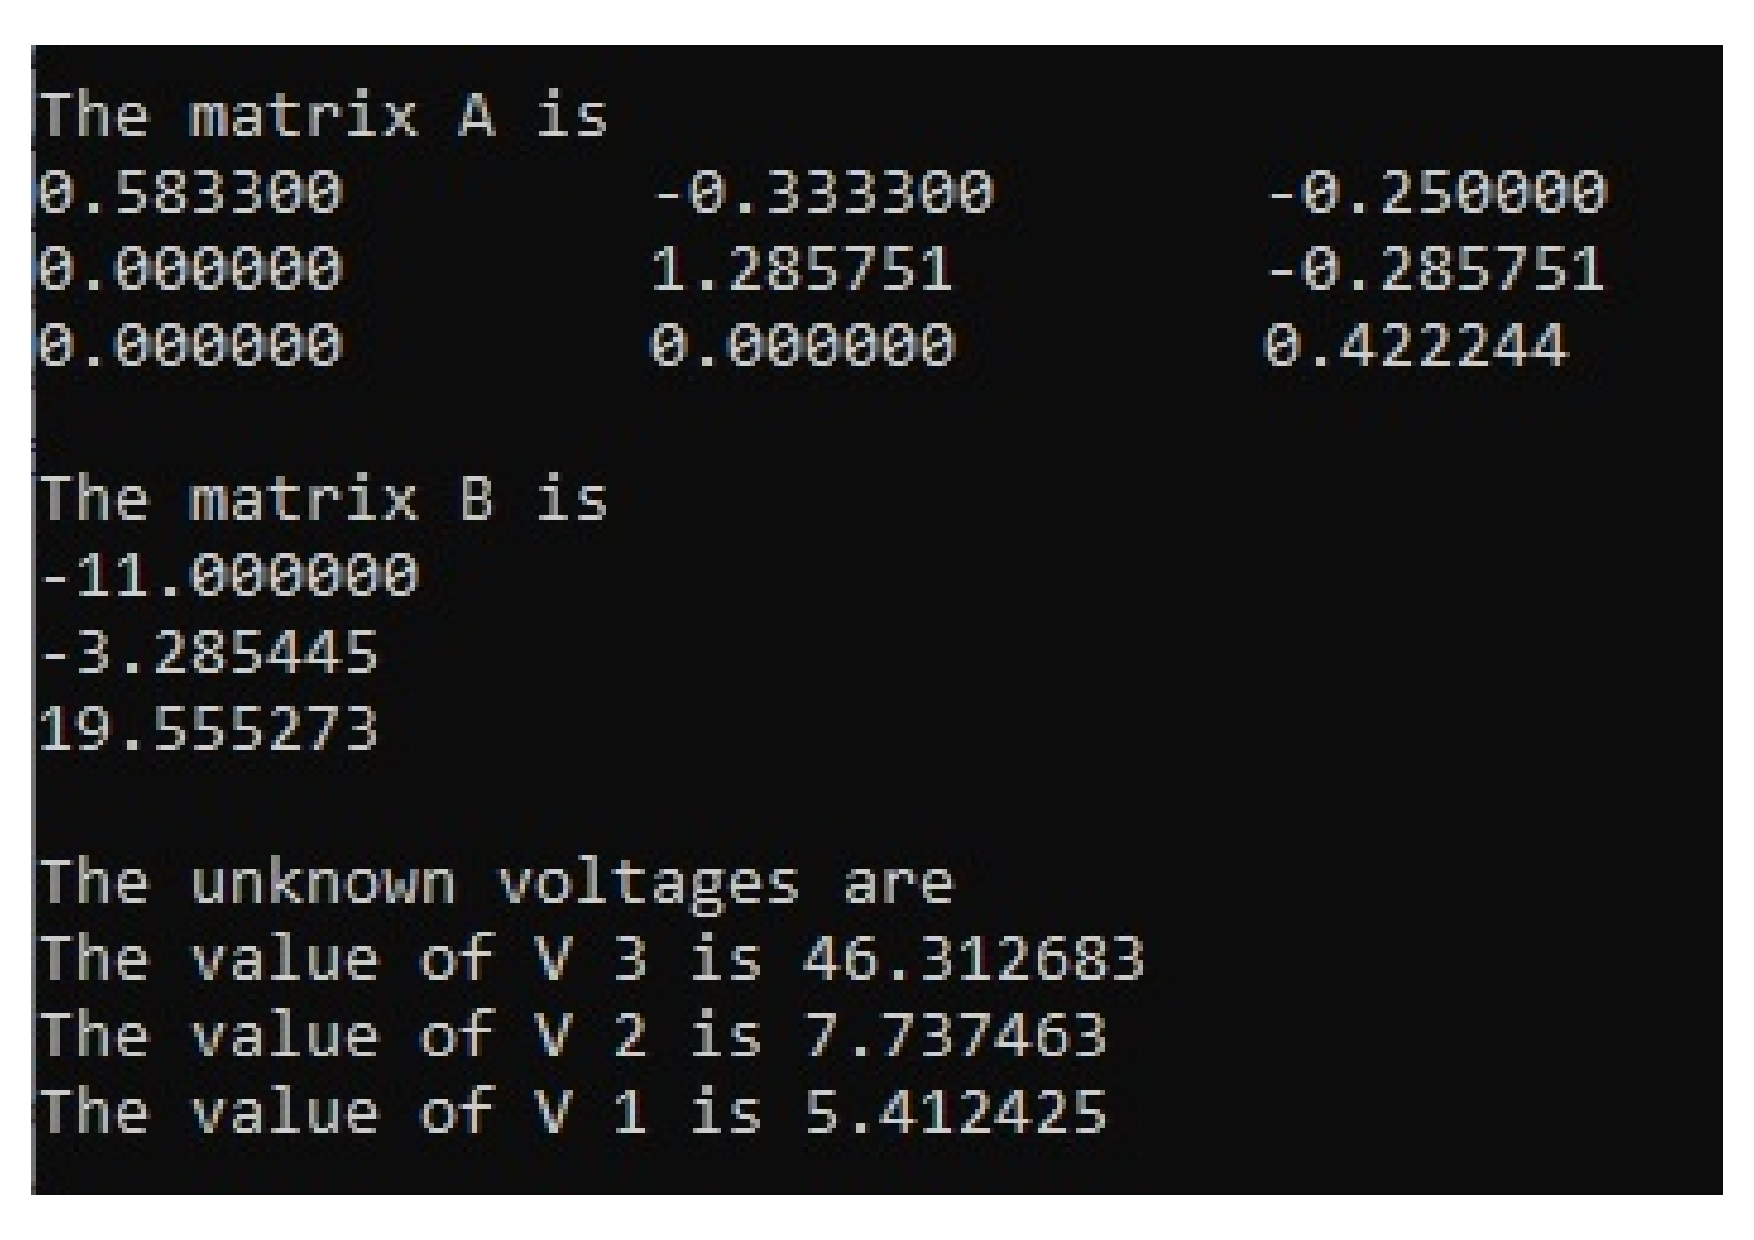
\includegraphics[width=0.9\textwidth]{Problem1.pdf}  
  	\caption{Screenshot showing the values of voltages V1, V2 and V3 along with Matrices A and B obtained after converting them into \textbf{Row Reduced Echelon Form}}
  	\label{fig:q12} 
\end{figure}


%%%%%%%%%%%%%%%%%%%%%%%%%%%%%%%%%%%%%%%%%%%%%%%%%%%%%%

\subsection{Inferences}

I deduce the following inferences from this problem :
\begin{itemize}
    \item [1] In this problem, the Gaussian Elimination gives accurate results. This need not be the case with all system of linear equations. 
    \item [2] Gaussian Elimination is a technique through which we can find results of a system of linear equations that are not ill-conditioned. The same holds true that Gaussian Elimination works only when the system of linear equations possess a unique solution.
    \item [3] Some amount of caution should be exercised in noting that the code could be modified to handle system of linear equations possessing infinite or zero solution by checking the determinant of the square matrix (if number of variables equals the number of equations) or otherwise, its rank.
    \item [4] The LU Decomposition (described in Problem 2) could be taken as a substitute for the normal Gauss Elimination as the former's results are generally more dependable. 
    \item [5] \label{Example} I shall demonstrate how the Gaussian Elimination fails to converge to the \textbf{right answer} in an \textbf{ill-conditioned system}. \\
    Consider the system of equations 
    \begin{equation}
         0.143 x + 0.357 y + 2.01 z = -5.173 
    \end{equation}
    \begin{equation}
         -1.31 x + 0.911 y + 1.99 z = -5.458 
    \end{equation}
    \begin{equation}
         11.2 x - 4.30 y - 0.605 z = 4.415  
    \end{equation}
    
    Gaussian Elimination in its present form gives the following output 
    \begin{itemize}
        \item [1] x = -0.950
        \item [2] y = -2.82
        \item [3] z = -2.00
    \end{itemize}
    
    But the solutions are trivial 
    \begin{itemize}
        \item [1] x = 1.00
        \item [2] y = 2.00
        \item [3] z = -3.00
    \end{itemize}
    
    Gaussian Elimination fails by a huge margin !!!!
    
    \item [6] Gauss Elimination, generally, fails in the following four situations
    \begin{itemize}
        \item [a] Division by zero
        \item [b] Round Off Errors
        \item [c] Ill-Conditioned System
        \item [d] Singular Systems
    \end{itemize}
    
    \item [7] The overall time complexity of Gauss Elimination comes out to be ${\frac{2n^3}{3} + O(n^2)}$
    \item [8] I shall mention few ideas through which we can tackle the above mentioned problems in Sub-Section ~\ref{alt:Alternative}
\end{itemize}

%%%%%%%%%%%%%%%%%%%%%%%%%%%%%%%%%%%%%%%%%%%%%%%%%%%%%%

\subsection{Code}
The code used for the experiments is mentioned in Listing~\ref{listing:1}. 

\inputminted[breaklines,
 mathescape,
 linenos,
 numbersep=5pt,
 frame=single,
 numbersep=5pt,
 xleftmargin=0pt]{c}{A4P1.c}
 \captionof{listing}{Code snippet used in the experiment.}
\label{listing:1}

%%%%%%%%%%%%%%%%%%%%%%%%%%%%%%%%%%%%%%%%%%%%%%%%%%%%%%

\subsection{Contributions}
In the above problem, \textit{my original contributions} are - 
\begin{itemize}
    \item Designing of the Algorithm and Code
    \item Tabulation of Results
    \item Drawing conclusions by looking at the Result obtained.
    \item Writing the report in LaTeX. 
\end{itemize}

%%%%%%%%%%%%%%%%%%%%%%%%%%%%%%%%%%%%%%%%%%%%%%%%%%%%%%

\subsection{Alternate Methods}
\label{alt:Alternative}
\begin{itemize}
    \item [1] Checking determinant/ rank at the start or avoiding run time errors like division by zero can serve as a quality-check at the beginning. 
    \item [2] Using more significant figures can reduce propagation of error. 
    \item [3] \href{https://web.mit.edu/10.001/Web/Course_Notes/GaussElimPivoting.html}{Gaussian Method with Pivoting} is one method that serves its purpose better than the Naive Gaussian Elimination. 
    \item [4] Scaling the equations is one strategy programmers use to tackle the situations described in Section ~\ref{Example}
    \item [5] \href{https://en.wikipedia.org/wiki/LU_decomposition}{The LU Decomposition} is a suitable alternative to the Gaussian Elimination. 
    \item [6] \href{https://math.libretexts.org/Bookshelves/Applied_Mathematics/Applied_Finite_Mathematics_(Sekhon_and_Bloom)/02%3A_Matrices/2.02%3A_Systems_of_Linear_Equations_and_the_Gauss-Jordan_Method}{The Gauss-Jordan Method} is an improvisation of the Gaussian Elimination technique by using an \textbf{Augmented Matrix} rather than a normal square matrix. 
    \item [7] If the matrix A has some special structure, this can be exploited to obtain faster or more accurate algorithms. For instance, systems with a symmetric positive definite matrix can be solved twice as fast with the \href{https://en.wikipedia.org/wiki/Cholesky_decomposition}{Cholesky decomposition}. \href{https://en.wikipedia.org/wiki/Levinson_recursion}{Levinson recursion} is a fast method for \href{https://en.wikipedia.org/wiki/Toeplitz_matrix}{Toeplitz matrices}. Special methods exist also for matrices with many zero elements which appear often in applications.
\end{itemize}

\newpage
%%%%%%%%%% END OF QUESTION 1 %%%%%%%%%%%%%%%%%%%
\section{Problem 2}
\noindent With modern networking environments becoming increasingly interconnected, the users' information is exposed to a lot of risks. Safely transmitting information, therefore becomes crucial. The two principles adopted for this purpose are called encoding (convert the original message to some secret message) and decoding (convert the secret message back to the original message). Some methods use matrices as part of the encoding and decoding processes.

\begin{figure}[h]
    \centering
    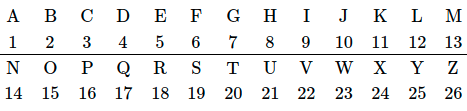
\includegraphics[scale = 0.5]{mapping.png}
    \caption{Mapping scheme for encoding messages}
    \label{fig:map}
\end{figure}

\begin{figure}[h]
    \centering
    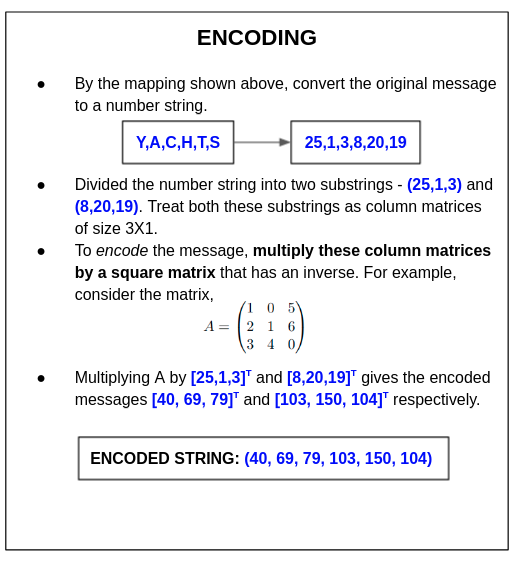
\includegraphics[scale = 0.55]{enc.png}
    \caption{Encoding messages}
    \label{fig:enc}
\end{figure}

\begin{figure}[H]
    \centering
    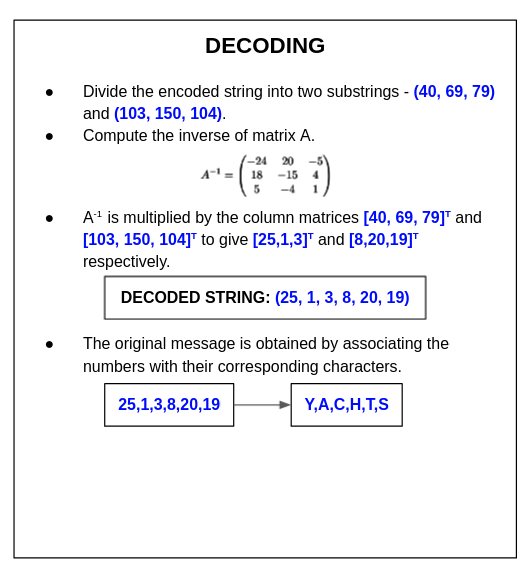
\includegraphics[scale = 0.55]{dec.png}
    \caption{Decoding messages}
    \label{fig:dec}
\end{figure}

\noindent For the remainder of this problem, we assume that the messages are character strings constructed from the set \{A, B, C, \ldots Z\}. The string of characters A to Z are mapped to integers $0$ to $26$ using the correspondence shown in Fig.~\ref{fig:map}. Note that the \textbf{blank space} character is mapped to \textbf{$27$}. The procedure for encoding and decoding messages is outlined in Fig.~\ref{fig:enc} and Fig.~\ref{fig:dec}. Use the same to solve the following parts:

\begin{itemize}
    \item [(a)] Find the inverse of the matrix $M$ using LU decomposition. Follow Example 10.3 on Page 284 from Steven Chapra to solve this problem. Paste a screenshot of the matrices $L$, $U$ and $M^{-1}$. 
    \vspace{-1}
    \begin{equation*}
    M = 
    \begin{pmatrix}
     1 & 4 & -3\\
     -2 & 8 & 5\\
     3 & 4 & 7
    \end{pmatrix}
    \end{equation*}
    
    \item [(b)] For the given \textbf{encoded} strings, determine the original message that was sent. In other words, multiply each column matrix by $M^{-1}$ and associate the numbers in the resulting column matrices with their respective characters. You may write a function to represent the character-number mapping and print the decoded message. In your report, paste a screenshot of the output displayed in your console. 
    
    \begin{itemize}
        \item [1] $[26, 115, 134]^T$, $[-16, 39, 88]^T$
        \item [2] $[7, 203, 269]^T$, $[-4, 269, 276]^T$, $[-20, 42, 156]^T$, $[-27, 116, 167]^T$
    \end{itemize}
    
\end{itemize}

\subsection{Approach}

Here I shall use the concept of LU decomposition of matrices to decompose a matrix M into a lower triangular matrix L and an upper triangular matrix U and hence obtain its inverse $M^{-1}$.
Also, it is well known beforehand that the matrix M is non-singular and is thus, invertible. 
I shall use the matrix $M^{-1}$ to find the decoded message. 

%%%%%%%%%%%%%%%%%%%%%%%%%%%%%%%%%%%%%%%%%%%%%%%%%%%%%%

\subsection{Algorithm}
In this section, I present the pseudocode/flowchart of the algorithm used to solve the problem.

The pseudocode for the summation is provided in Algorithm~\ref{alg2}.
\begin{center}
\begin{algorithm}[H]\label{alg2}

\SetAlgoLined
{
\underline{\textbf{LU Decomposition}} \\
{
\For{$k=0$ to $2$}{
   \For{$i=k+1$ to 3}{
      $r_{ik}$ $\gets$ $\frac{a_{ik}}{a_{kk}}$ \\
      \For{$j=k+1$ to 3}{
         $a_{ij}$ $\gets$ $a_{ij} - r_{ik}a_{kj}$ \\
      }
      $b_{i}$ $\gets$ $b_{i}-r_{ik}b{k}$ \\
      $L_{ik}$ $\gets$ $r_{ik}$ \\ 
   }
}
Set $A_{10}=A_{20}=A_{21}=0$ \\
\For{$i=0$ to 3}{
   \For{$j=0$ to 3}{
        \If{i==j}{
          Set $L_{ij}=1$ \\
        }
        \If{j>i}{
          Set $L_{ij}=0$ \\
        }
   }
}
}
\underline{\textbf{Forward Substitution}} \\ 
  Set $y_1$ = $b_1/l_{11}$ \\
  \For{$i=2$ to n}{
     $y_i$ $\gets$ $(b_i - \sum_{j=1}^{i-1}l_{ij}y_{j})/l_{ii}$
  }
\underline{\textbf{Back Substitution}} \\{
    Set $x_n = {y_n}/{u_{nn}}$ \\
    \For{$i=n-1$ to 1}{
      ${x_i \gets (y_i - \sum_{j=i+1}^{n}u_{ij}x_j)/u_{ii}}$
    }
}
}
 \caption{LU Decomposition}
\end{algorithm}    
\end{center}

%%%%%%%%%%%%%%%%%%%%%%%%%%%%%%%%%%%%%%%%%%%%%%%%%%%%%%
\subsection{Results}

In this section, I shall paste the screenshots of the Matrices obtained after LU Decomposition.  

The Matrices L,U and $M^{-1}$ have been shown in Figure~\ref{fig:q12}. 

After decoding the message, we obtain the answers for the problems (a) and (b) respectively as follows :
\begin{itemize}
    \item [(a)] IKIGAI
    \item [(b)] POWER RANGER
\end{itemize}
The screenshot for the same has been shown in Figure ~\ref{fig:q13}

\begin{figure}[!tbh]
  	\centering
  	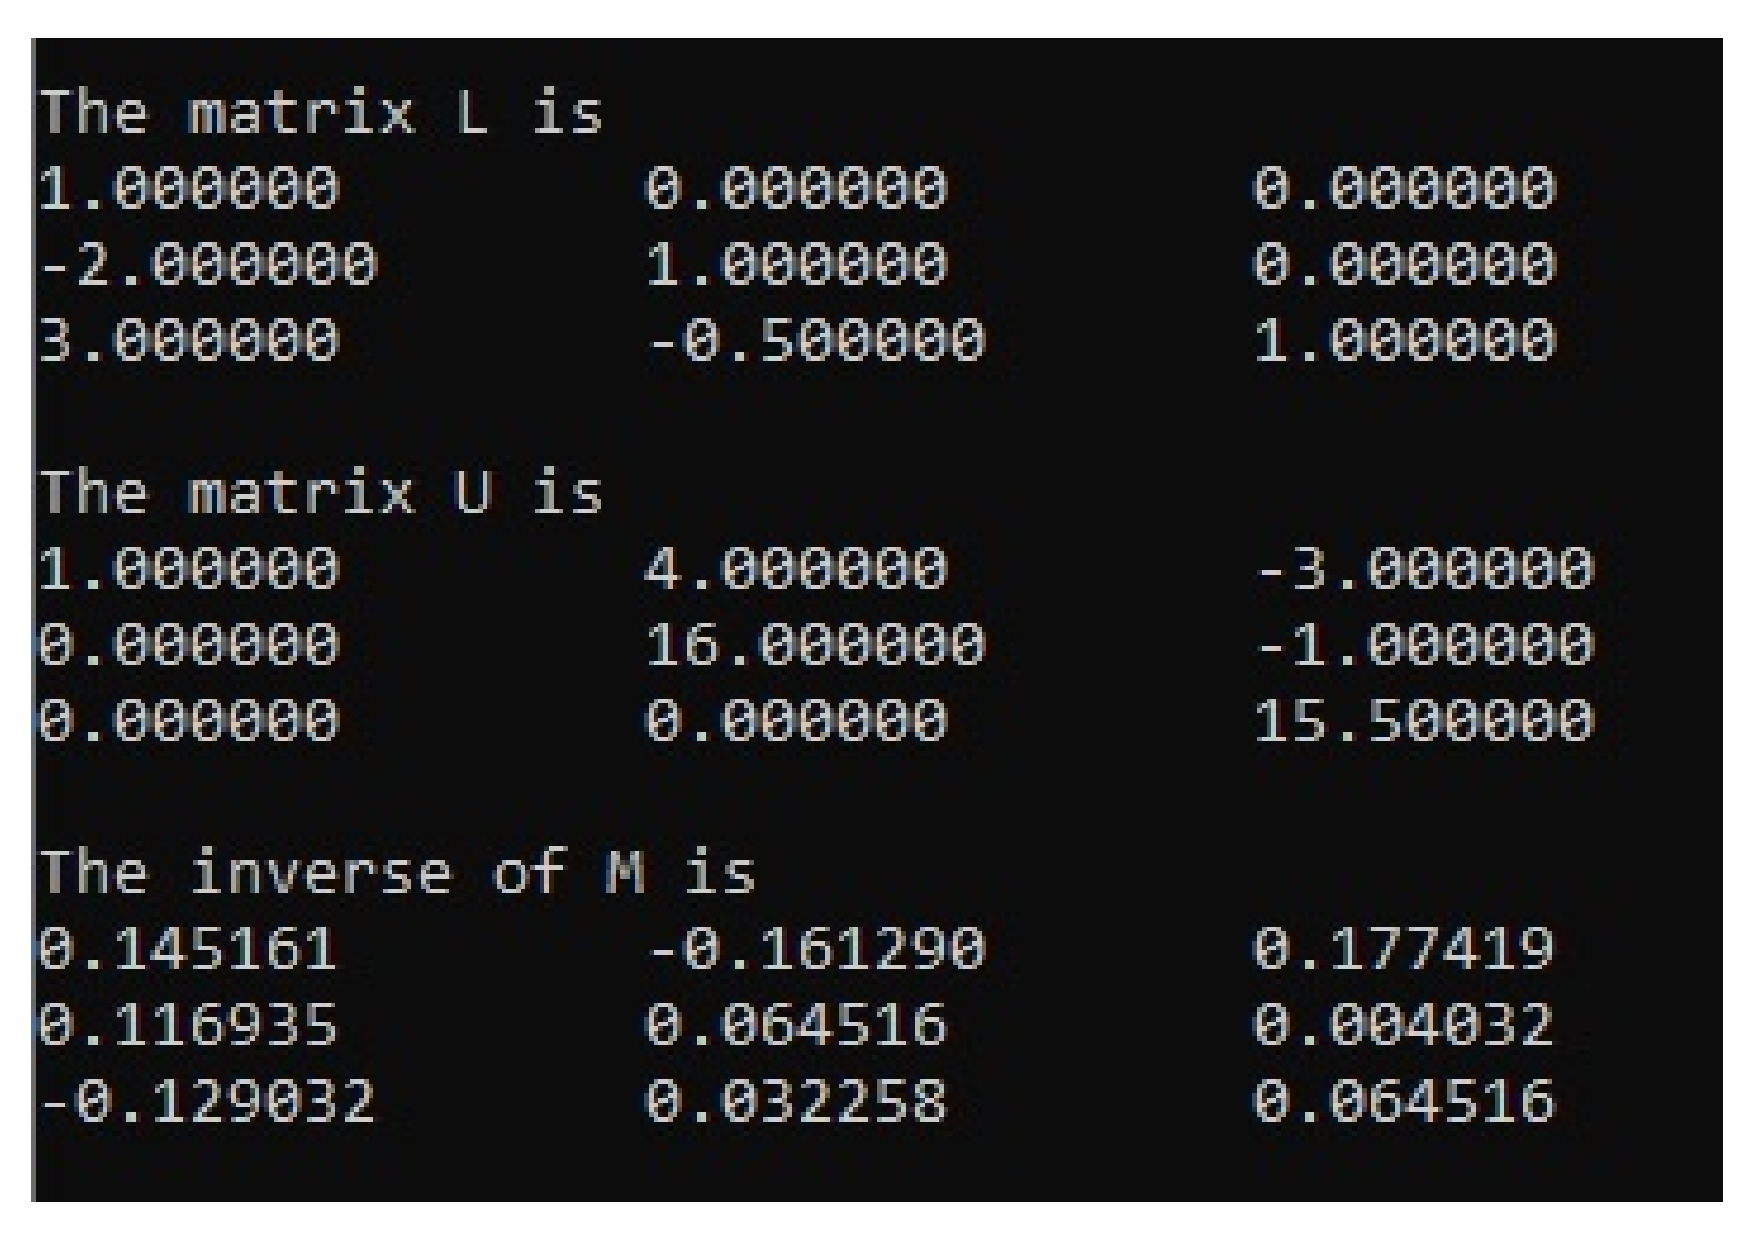
\includegraphics[width=0.9\textwidth]{Problem2.pdf}  
  	\caption{Screenshot showing the Matrices L, U and $M^{-1}$}
  	\label{fig:q12} 
\end{figure}

\begin{figure}[!tbh]
  	\centering
  	
\includegraphics[width=0.9\textwidth]{Problem2b.png}  
  	\caption{Screenshot showing the decoded messages}
  	\label{fig:q13} 
\end{figure}


%%%%%%%%%%%%%%%%%%%%%%%%%%%%%%%%%%%%%%%%%%%%%%%%%%%%%%

\subsection{Inferences}

I deduce the following inferences from this problem :
\begin{itemize}
    \item [1] The LU Decomposition is a reliable technique that can be used when the matrix B is different even though matrix A is the same. This serves as the basis of solving of linear systems in many engineering applications like solving Circuit equations and Image Processing
    \item [2] The LU Decomposition might turn out to be our best foot forward in case of very large matrices (of say order 1000 x 1000). In such situations, Gaussian Elimination is clearly out of the race as it cannot solve the system with a great efficiency. 
    \item [3] However, it may not be possible to write certain matrices of the form M = LU. This is true and care needs to be taken in solving such situations. 
    \item [4] The overall time-complexity of LU Decomposition comes out to be $\frac{n^3}{3} + O(n^2)$
    \item [5] A suitable analog of the LU Decomposition that comes handy in certain applications is \href{https://en.wikipedia.org/wiki/Crout_matrix_decomposition}{The Crout Decomposition}. It can be considered that both LU and Crout work on the same idea of decompsing a matrix M as a product of a lower triangular matrix L and upper triangular matrix U.
    \item [6] Not all matrices are invertible. We need to check for the same by either evaluating the determinant or the rank. 
    \item [7] In general, when the situation is ideal (unique solution exists), the LU Decomposition seems to be a good and reliable option when compared to the Gauss Elimination. 
    \item [8] When the system possesses zero solution or no solution, then this method fails. 
\end{itemize}

%%%%%%%%%%%%%%%%%%%%%%%%%%%%%%%%%%%%%%%%%%%%%%%%%%%%%%

\subsection{Code}
The code used for the problem is mentioned in Listing~\ref{listing:2}. 

\inputminted[breaklines,
 mathescape,
 linenos,
 numbersep=5pt,
 frame=single,
 numbersep=5pt,
 xleftmargin=0pt]{c}{A4P2.c}
 \captionof{listing}{Code snippet used in the experiment.}
\label{listing:2}

%%%%%%%%%%%%%%%%%%%%%%%%%%%%%%%%%%%%%%%%%%%%%%%%%%%%%%

\subsection{Contributions}
In the above problem, \textit{my original contributions} are - 
\begin{itemize}
    \item Designing of the Algorithm and Code
    \item Tabulation of Results
    \item Drawing conclusions by looking at the Result obtained.
    \item Writing the report in LaTeX. 
\end{itemize}

%%%%%%%%%%%%%%%%%%%%%%%%%%%%%%%%%%%%%%%%%%%%%%%%%%%%%%

\subsection{Alternate Methods}
\begin{itemize}
   \item [1] \href{https://math.libretexts.org/Bookshelves/Applied_Mathematics/Applied_Finite_Mathematics_(Sekhon_and_Bloom)/02%3A_Matrices/2.02%3A_Systems_of_Linear_Equations_and_the_Gauss-Jordan_Method}{The Gauss-Jordan Method} is an improvisation of the Gaussian Elimination technique by using an \textbf{Augmented Matrix} rather than a normal square matrix. 
    \item [2] If the matrix A has some special structure, this can be exploited to obtain faster or more accurate algorithms. For instance, systems with a symmetric positive definite matrix can be solved twice as fast with the \href{https://en.wikipedia.org/wiki/Cholesky_decomposition}{Cholesky decomposition}. \href{https://en.wikipedia.org/wiki/Levinson_recursion}{Levinson recursion} is a fast method for \href{https://en.wikipedia.org/wiki/Toeplitz_matrix}{Toeplitz matrices}. Special methods exist also for matrices with many zero elements which appear often in applications.
    \item [3] \href{https://en.wikipedia.org/wiki/Gauss%E2%80%93Seidel_method#:~:text=In%20numerical%20linear%20algebra%2C%20the,a%20system%20of%20linear%20equations.}{The Liebmann method} is a suitable alternative to the otherwise reliable LU Decomposition Algorithm. 
    \end{itemize}
% Uncomment the lines below to add references using bibtex.
% \bibliographystyle{plainnat}
% \bibliography{references}

\end{document}
